\chapter{Solution Design}

\section{Introduction}

Reviewing the image-based approaches for wheat disease identification helped highlight the various techniques and models used to tackle the challenge of accurate disease recognition. This review provided valuable insights into the strengths and limitations of existing methods, guiding the development of a more tailored and effective solution.

This chapter presents the design of our proposed solution for wheat disease detection and classification. It outlines the system architecture, the preparation of relevant datasets, and the deep learning models employed. In addition to the main classification module, the system includes two additional modules: one for insect pest detection, and another integrating a general-purpose AI assistant via an API to help guide users and enhance their experience. The chapter also describes the web platform developed to deploy the solution and make it accessible to end users.

\section{General design of the proposed solution}
Accurate detection of wheat diseases is essential for smart agriculture. While deep learning models show promise, many struggle with accurately predicting multiple disease classes. A major issue is the high false alarm rate, which incorrectly identifies healthy crops as diseased, leading to misdiagnosis, unnecessary interventions, and reduced trust in the system's reliability. Additionally, the similarity of symptoms across different fungal diseases often results in misclassification between disease types, which can cause farmers to choose inappropriate treatment methods, potentially worsening the situation or wasting resources.

The main goal of this work is to develop a robust deep learning solution capable of:
\begin{itemize}
    \item Detecting multiple wheat disease classes with high accuracy and recall, ensuring minimal false negatives (missed detections) and false positives (false alarms).
    \item Improving solution generalization across different environmental conditions (variations in lighting, backgrounds, and leaf positioning), image sources (e.g., drone, phone), and wheat varieties.
    \item Building an efficient solution suitable for integration into mobile or web applications for farmers.
\end{itemize}

To address the challenges identified during the literature review, our proposed classification solution leverages deep convolutional neural networks trained on high-resolution RGB images of wheat crops. The classification module is designed to accurately detect and distinguish between multiple wheat disease classes, even when symptoms appear visually similar. By carefully curating and augmenting the training dataset, we aim to improve model robustness against variations in lighting, image quality, background noise, and different wheat varieties. The system processes input images from diverse sources such as drones, cameras, or mobile phones, and outputs a reliable disease class prediction. This core classification module serves as the foundation of our approach, ensuring precision and scalability for real-world deployment.

To enrich the proposed solution and move toward a more holistic crop health monitoring system, additional modules were integrated into the system. One of these focuses on insect pest detection, as certain pests can be the primary cause of specific wheat diseases. Their early identification is crucial for addressing the root causes of infection and ensuring that treatment strategies target both symptoms and sources. Additionally, a general-purpose AI assistant was integrated via an API to support users by answering questions, guiding interpretation of results, and offering practical recommendations. Together with our proposed classification solution, these modules enhance the system’s ability to provide more accurate, timely, and context-aware support to farmers. Figure~\ref{fig:GlobalSys} illustrates the global design of the proposed solution, including the main classification module and the two complementary modules.
\begin{figure}[H] % 'H' needs \usepackage{float}
    \centering
    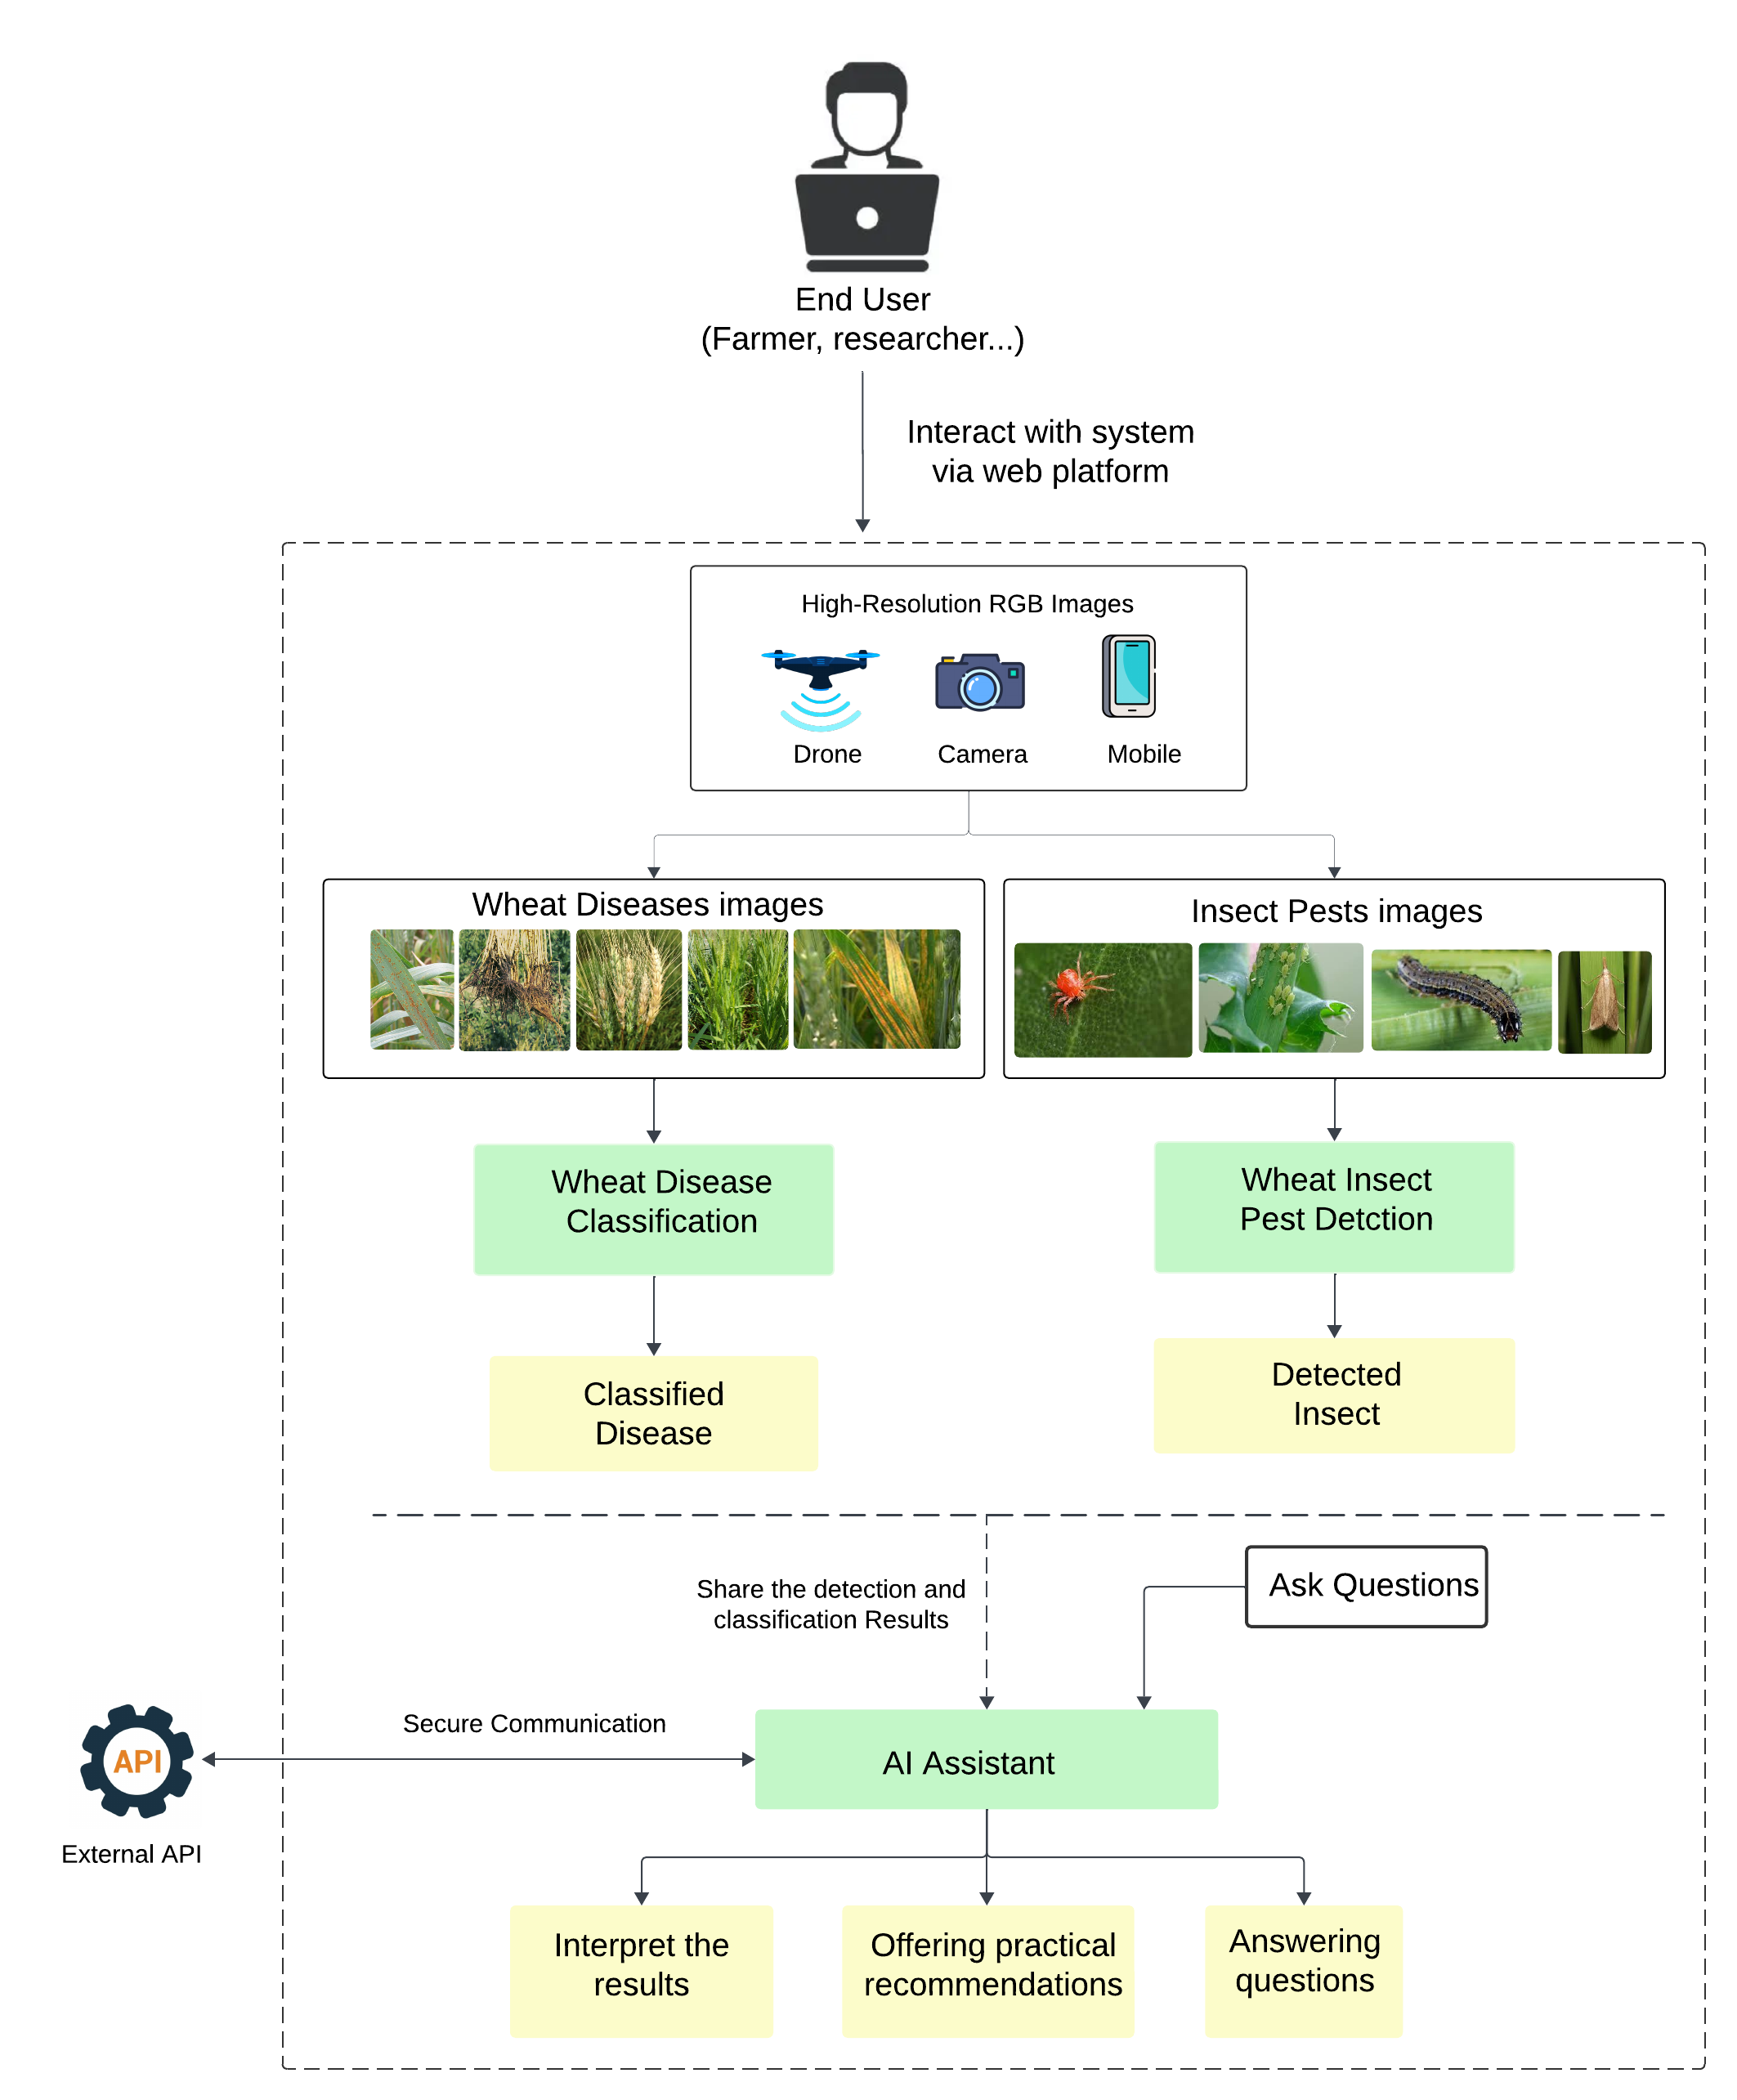
\includegraphics[width=0.9\textwidth]{chapters/chapter4/images/Figure00.png}
    \caption{Block Diagram of the Proposed Multi-Module Wheat Monitoring System.}
    \label{fig:GlobalSys}
\end{figure}

\section{Detailed design of the proposed solution: Wheat disease classification}
This section outlines the methodology adopted for detecting and classifying wheat diseases, detailing the system's objectives, overall architecture, dataset design, and the models used in various classification scenarios.

\subsection{Global architecture overview}
The proposed solution adopts a two-stage classification pipeline to ensure both high accuracy and interpretability. Once the input image is preprocessed, it is first passed through a binary classification model to determine the presence of disease. If the wheat plant is identified as diseased, a second model performs detailed diagnosis to identify the specific condition (See Figure ~\ref{fig:HierarchicalSystem}). The structure is described as follows:
\begin{itemize} 
    \item \textbf{Model 1 – Binary Classification:} This initial model determines whether the wheat plant is healthy or diseased. If the plant is classified as healthy, the system outputs a \textit{"Healthy"} result and halts further processing.

    \item \textbf{Model 2 – Multiclass Classification:} If a disease is detected, this model takes over to identify the exact type of disease. It can classify the image into one of eight common wheat diseases: \textit{Yellow Rust}, \textit{Brown Rust}, \textit{Stem Rust}, \textit{Powdery Mildew}, \textit{Loose Smut}, \textit{Septoria}, \textit{Fusarium},  \textit{Tan Spot} and \textit{Common Root Rot}.
\end{itemize}
% \subsection{System Strengths and Advantages}

% The proposed system demonstrates several strong points that contribute to its effectiveness:
% \begin{itemize}
%     \item \textbf{Efficient Decision-Making:} The step-by-step structure simplifies complex classification tasks and improves accuracy.
%     \item \textbf{Improved Accuracy Through Specialisation:} Each model handles a narrower, well-defined task, resulting in better training outcomes and higher performance for specific disease groups.
%     \item \textbf{Modularity:} Models are independent and can be updated, retrained, or replaced individually without affecting the entire system.
%     \item \textbf{Better Interpretability:} The hierarchical decision flow is transparent, making it easier to understand, explain, and debug system outputs.
%     \item \textbf{Scalability:} The architecture allows for easy integration of new disease categories or additional models without major system changes.
% \end{itemize}

\begin{figure}[H] % 'H' needs \usepackage{float}
    \centering
    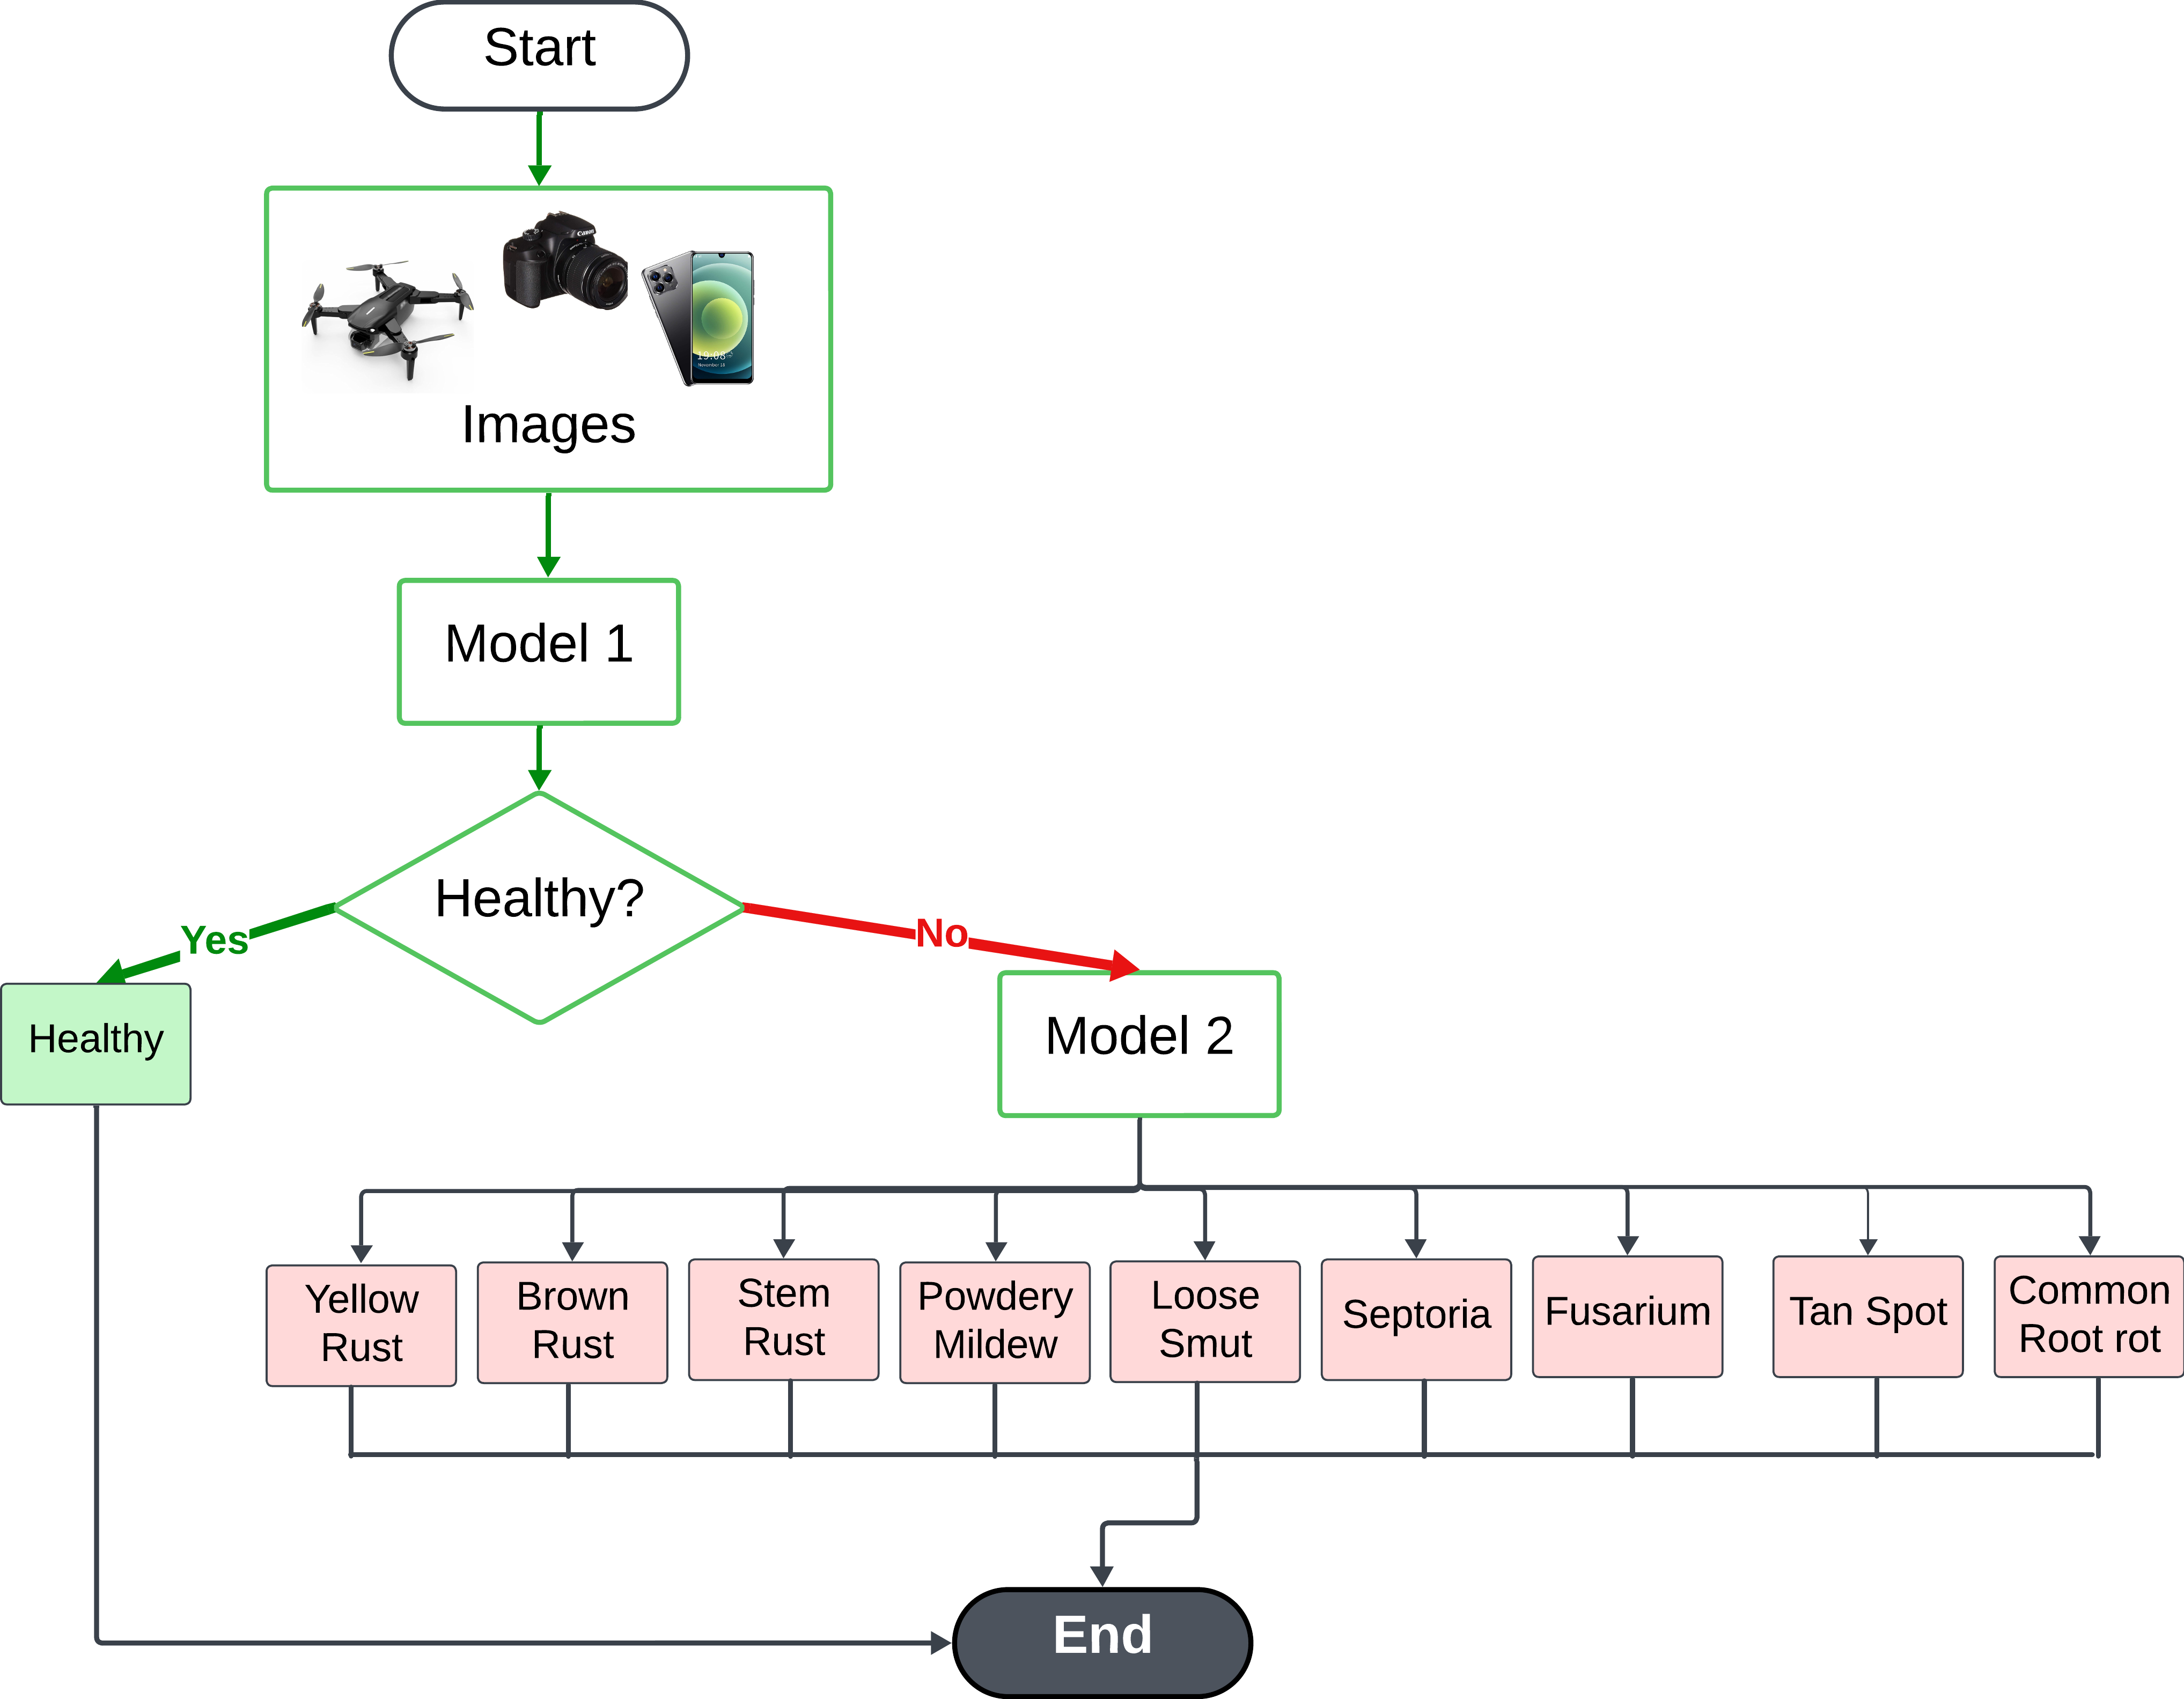
\includegraphics[width=0.9\textwidth]{chapters/chapter4/images/Figure01.png}
    \caption{Hierarchical system for wheat disease classification.}
    \label{fig:HierarchicalSystem}
\end{figure}

This two-tiered model significantly improves both efficiency and classification performance by:

\begin{itemize}
    \item \textbf{Reducing computational complexity:} Only diseased samples undergo detailed classification, which minimizes unnecessary computation.
    
    \item \textbf{Enhancing modularity and scalability:} Each model can be updated or improved independently, allowing for flexible system maintenance and upgrades.
    
    \item \textbf{Promoting interpretability:} The decision-making process is divided into logically distinct stages, making it easier to understand and validate each step.
\end{itemize}

Such a modular approach ensures robust, accurate, and adaptable disease detection, making the system suitable for real-world deployment in precision agriculture and smart farming applications.




\subsection{Wheat disease dataset construction}
Various public datasets for wheat disease detection are available online through platforms like Kaggle, GitHub, and Google Drive. These datasets typically contain images representing a few disease classes, but the image counts and quality vary significantly. Common issues include low-resolution or blurred images, misclassified or irrelevant samples, redundant (duplicate) images, and limited class diversity often covering only two to four disease types. Additionally, some datasets contain images that are not only unrelated to the disease but also have no clear connection to wheat itself, which can introduce noise and reduce model performance. Moreover, most images are captured at close range, which limits the model’s ability to generalize to field-level scenarios,  such as those involving RGB drone imagery.
\begin{table}[htbp]
    \caption{Overview of used wheat disease datasets}
    \centering
    \resizebox{\textwidth}{!}{%
    \begin{tabular}{|p{4cm}|p{2cm}|p{6cm}|p{3.5cm}|}
    \hline
    \textbf{Dataset} & \textbf{Source} & \textbf{Classes} & \textbf{Size} \\
    \hline
    Wheat Leaf Dataset & Mendeley Data & Healthy (102), Stripe Rust (208), Septoria (97) & 407 images \\
    \hline
    Wheat Disease Detection & Kaggle & Healthy (1116), Yellow Rust (924), Brown Rust (902) & 2942 images \\
    \hline
    Wheat Fungi Diseases Dataset (WFD 2020) & \parencite{genaev2021} &Healthy (517), Yellow Rust (457), Stem Rust(388),  Septoria (185), Leaf Rust (655), Powdery Mildew (277), seedling (255) & 2734 images \\
    \hline
    CGIAR & Kaggle & Healthy (142), Leaf Rust (358), Stem Rust (376) & 876 images \\
    \hline
    LWDCD 2020 & Google Drive & Crown and Root Rot (1040), Fusarium Head Blight (1270), Healthy (1280), Leaf Rust (1620) & 5210 images \\
    \hline
    Wheat Disease Dataset WDD 2017 & Kaggle & Brown Rust (166), Healthy (242), Loose Smut (99), Septoria (34), Yellow Rust (195) & 736 images \\
    \hline
    \end{tabular}%
    }
    \label{tab:wheat-datasets}
\end{table}

To overcome the limitations of existing datasets, we constructed a custom wheat disease dataset by carefully curating and filtering images from multiple publicly available sources (Table~\ref{tab:wheat-datasets}). This involved eliminating low-quality or irrelevant samples, correcting mislabeled entries, and ensuring visual diversity, particularly in terms of image acquisition angles and capture distances (e.g., close-up and aerial views). The primary objective was to build a robust and representative dataset capable of supporting accurate and generalizable classification under diverse real-world conditions. Our final dataset comprises 4,215 images spanning ten distinct classes: Healthy, Yellow Rust, Stem Rust, Brown Rust, Powdery Mildew, Septoria, Loose Smut, Fusarium, Tan Spot and Common Root Rot (Figure~\ref{fig:ourcustomdataset}).

\begin{figure}[H] % 'H' needs \usepackage{float}
    \centering
    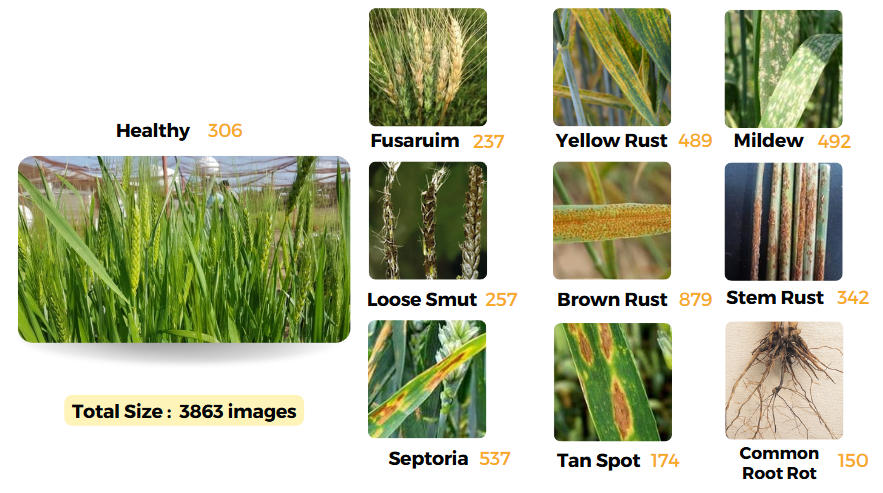
\includegraphics[width=0.9\textwidth]{chapters/chapter4/images/Figure02.png}
    \caption{Sample images from our custom dataset.}
    \label{fig:ourcustomdataset}
\end{figure}

To facilitate the development and training of the hierarchical classification system, the dataset was strategically partitioned into two subsets: D1 and D2, tailored for Model 1 and Model 2, respectively. D1 supports Model 1, a binary classifier designed to distinguish between healthy and unhealthy wheat plants. To ensure class balance, 410 images labeled as "Not Healthy" were randomly sampled from the nine disease categories and paired with 381 "Healthy" images. In contrast, D2 was constructed for Model 2, the multi-class classifier, and includes all disease classes except the "Healthy" category.

\subsection{Binary classification model}
The binary classification architecture, illustrated in Figure~\ref{fig:binaryClassification}, comprises three main stages: data preparation, feature extraction, and classification.

\begin{figure}[H] % 'H' needs \usepackage{float}
    \centering
    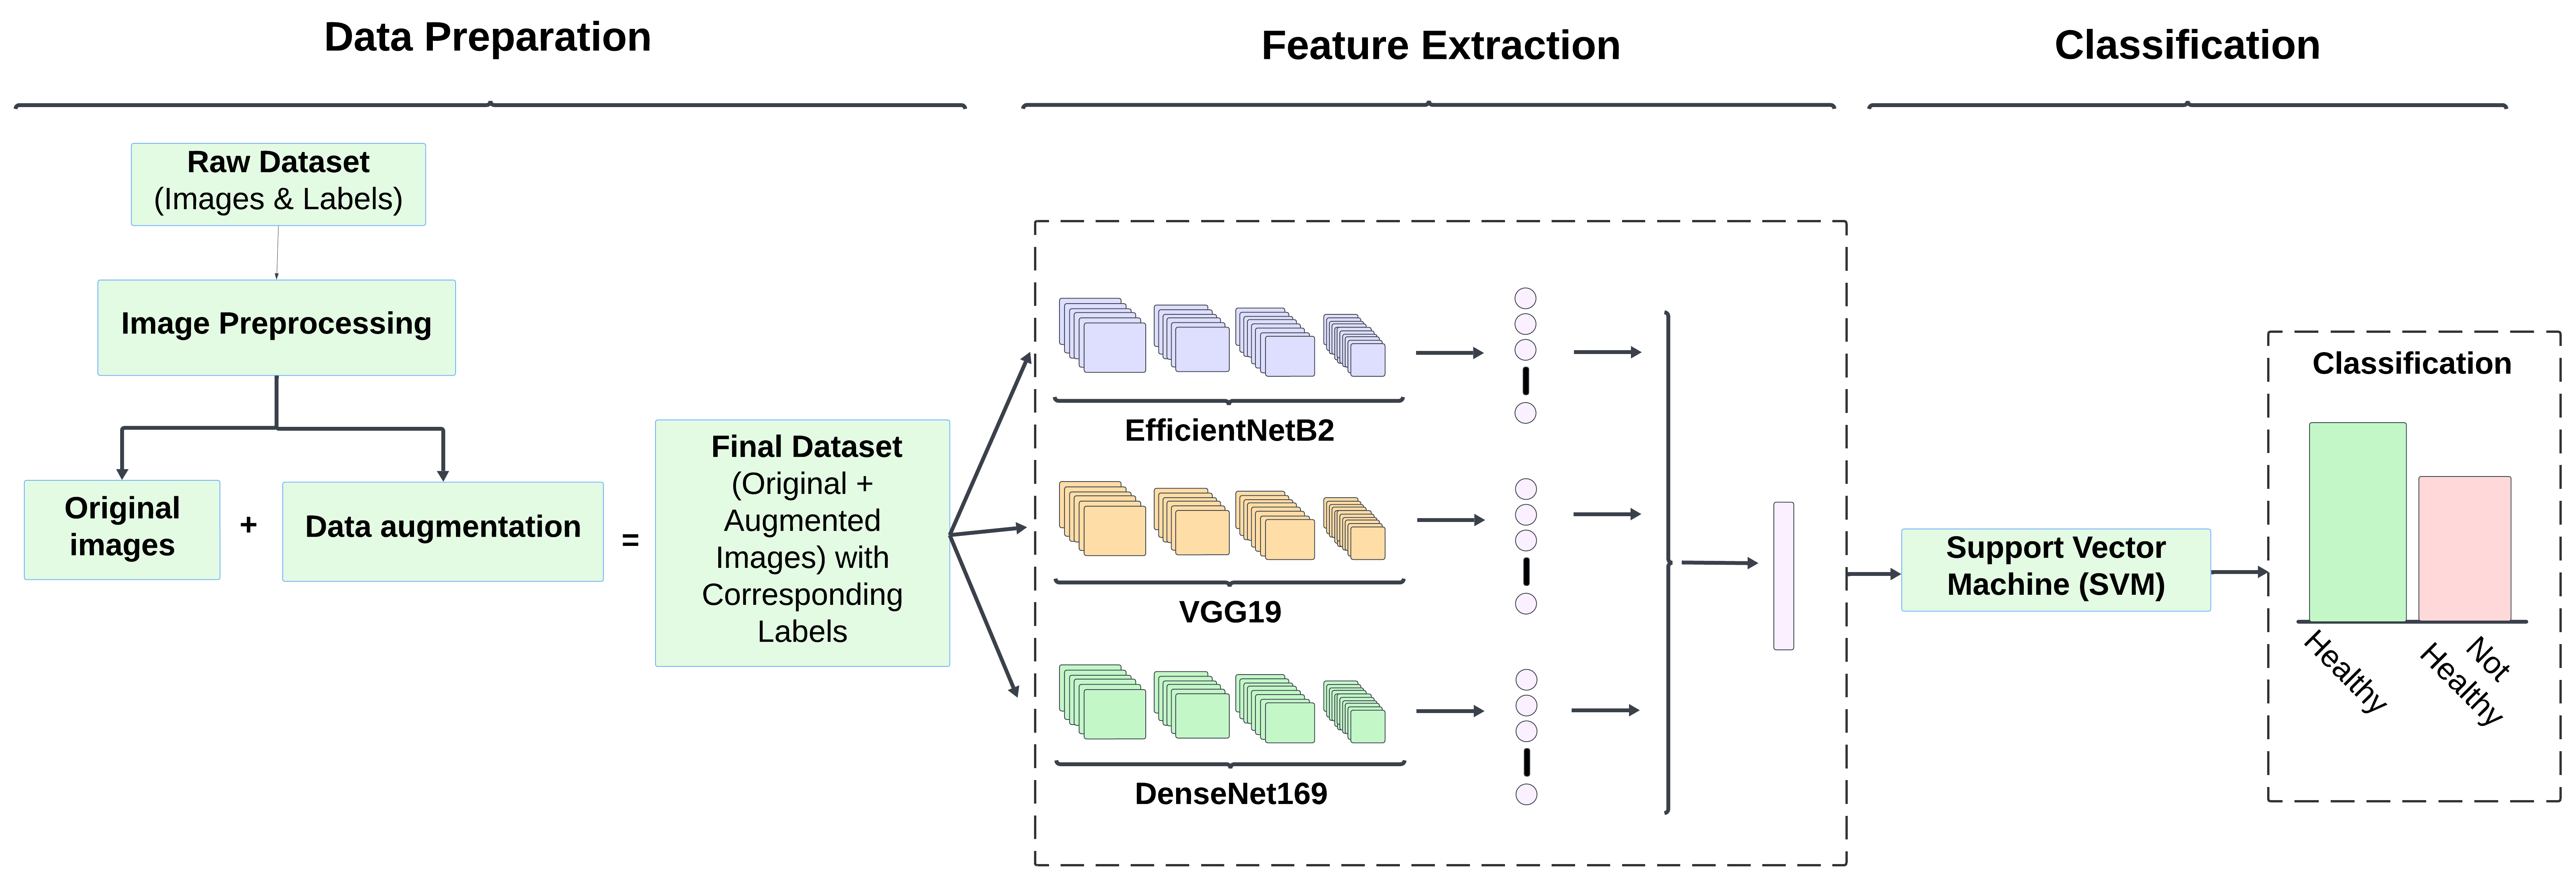
\includegraphics[width=1\textwidth]{chapters/chapter4/images/Figure03.png}
    \caption{Architecture of the binary classification model.}
    \label{fig:binaryClassification}
\end{figure}


\subsubsection{Data preparation:} The raw dataset undergoes preprocessing to standardize image quality, followed by data augmentation techniques to improve variability and generalizability. The final dataset combines both original and augmented images, each with corresponding labels, to ensure a balanced and enriched training set.
\vspace{0.3cm}
\subsubsection{Feature Extraction:} The final dataset is fed into four state-of-the-art pre-trained convolutional neural networks (CNNs): EfficientNetB2, VGG19, and DenseNet169. Each model extracts high-level features from the final layers of its architecture, typically from the global average pooling or fully connected layers. These features are then flattened and concatenated to form a comprehensive high-dimensional feature vector, capturing diverse and complementary visual representations for improved classification performance.
\vspace{0.3cm}
\subsubsection{Classification:} 
The concatenated feature vectors are passed to a Support Vector Machine (SVM), a robust and well-established traditional classifier, to perform binary classification. The model outputs one of two labels: “Healthy” or “Not Healthy,” indicating the presence or absence of disease in the wheat plant.

\textbf{Support Vector Machine (SVM)} is a powerful supervised machine learning algorithm widely used for classification and regression tasks due to its efficiency and ability to manage high-dimensional data. At its core, SVM aims to find the optimal hyperplane that best separates data points from two classes by maximizing the margin, the distance between the hyperplane and the nearest data points, known as support vectors. When data is not linearly separable, SVM applies the "kernel trick" to map inputs into a higher-dimensional space where a linear separation becomes feasible (Figure~\ref{fig:SVM}); common kernel functions include linear, polynomial, radial basis function (RBF), and sigmoid \parencite{guido2024}.

\begin{figure}[H] % 'H' needs \usepackage{float}
    \centering
    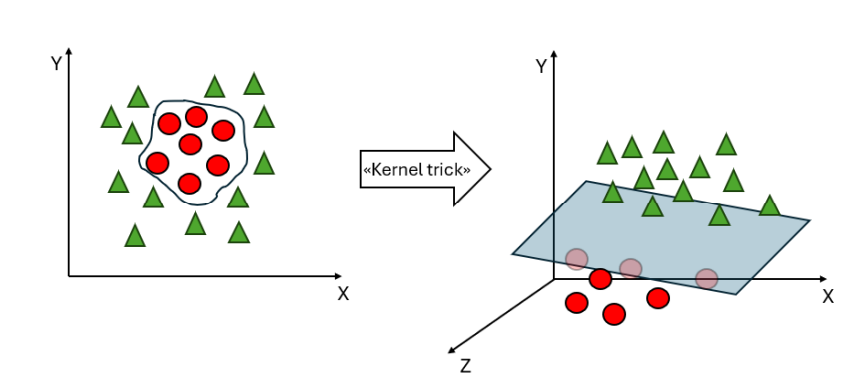
\includegraphics[width=0.9\textwidth]{chapters/chapter4/images/Figure04.png}
    \caption{An example of the “kernel trick” \parencite{guido2024}.}
    \label{fig:SVM}
\end{figure}



\subsection{Multi-class classification Model}
Model 2 is a deep learning-based multi-class classification architecture designed to detect various wheat diseases from input images. It incorporates essential components such as data preprocessing techniques, a powerful feature extractor (ResNet-50), an attention mechanism, and a fully connected classification head to improve performance. The overall architecture and data flow of the model are illustrated in Figure~\ref{fig:Multiclassclassification}.

\begin{figure}[H] % 'H' needs \usepackage{float}
    \centering
    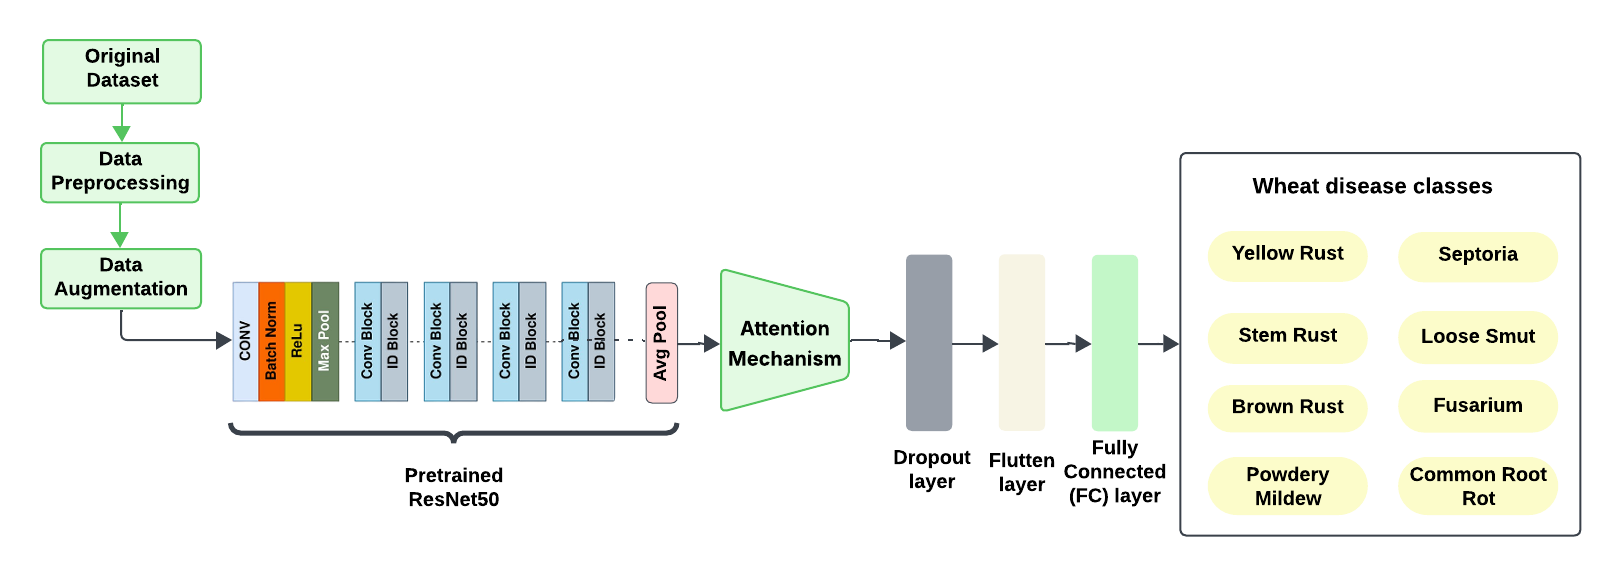
\includegraphics[width=1\textwidth]{chapters/chapter4/images/Figure05.png}
    \caption{Architecture of the multi-class wheat disease classification model.}
    \label{fig:Multiclassclassification}
\end{figure}


\textbf{Data preprocessing:} This stage applies standard image preprocessing techniques, including resizing to a uniform input size, random cropping to introduce spatial variability, and standard normalization to scale pixel values. These steps ensure consistency across the dataset and improve the model’s ability to generalize by reducing input variance.

\textbf{Data augmentation:} A diverse set of transformations was applied, including random cropping, flipping, rotation, color adjustments, brightness and contrast changes, blurring, and geometric distortions. These augmentations simulate real-world variations in lighting, orientation, and image quality, helping the model learn more discriminative features and reducing the risk of overfitting.

\textbf{Feature extraction with pretrained ResNet-50:} At the core of the architecture lies a pretrained \textbf{ResNet-50} model, used as a feature extractor:
\begin{itemize}
    \item The image data flows through several convolutional layers (Conv Blocks), each followed by identity blocks (ID Blocks), ReLU activations, batch normalization, and max pooling.
    \item The pretrained weights from ImageNet allow the network to extract rich, hierarchical image features without requiring training from scratch.
    \item An average pooling layer summarizes the extracted features, reducing spatial dimensions and focusing on high-level representations.
\end{itemize}

\textbf{Attention Mechanism:} 
To enhance the model’s ability to capture the most relevant and discriminative features in an image, we integrate the Efficient Channel Attention (ECA) mechanism after the feature extraction stage. Unlike traditional convolutional layers that process all channels equally, ECA dynamically emphasizes the most informative channels in the feature maps.


The ECA module operates on a feature map of dimensions \( H \times W \times C \), where \( H \) (High) and \( W \) (Width) represent the spatial dimensions and \( C \) the number of channels. First, it applies global average pooling across the spatial dimensions, transforming the input into a compact \( 1 \times 1 \times C \) vector that captures the average response of each channel. This vector is then passed through a lightweight 1D convolution with a small kernel size to model local cross-channel interactions without dimensionality reduction, the resulting attention weights are then applied to the original channels through element-wise multiplication, effectively boosting salient features while suppressing less relevant ones (Figure\ref{fig:ECA}). This approach enhances the model's focus on disease-related visual cues, such as subtle lesions, discolorations, or texture anomalies, which are critical for accurate classification. Importantly, ECA achieves this with minimal computational overhead, making it ideal for lightweight and real-time applications \parencite{hao2024squeezenet}.

\begin{figure}[H]
    \centering
    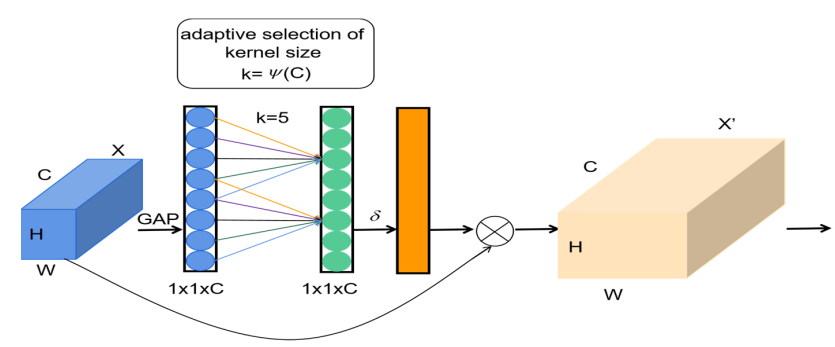
\includegraphics[width=0.8\textwidth]{appendices/images/FigureA9.png}
    \caption{ECA mechanism module \protect\parencite{hao2024squeezenet}.}
    \label{fig:ECA}
\end{figure}



\textbf{Classification head:} After applying attention, the model includes a classification head that consists of:
\begin{itemize}
    \item \textbf{Dropout layer:} Helps prevent overfitting by randomly disabling some neurons during training.
    \item \textbf{Flatten layer:} Converts the 2D feature maps into a 1D vector.
    \item \textbf{Fully connected (FC) layer:} A linear layer that maps the extracted and attended features to class logits.
\end{itemize}


\section{Extending the proposed solution with insect pest detection and AI assistant for Proactive Intervention}
To enhance the overall effectiveness and practical relevance of the proposed wheat disease classification system, two additional modules were integrated into the web application: insect pest detection and an AI assistant. These enhancements extend the system’s capabilities from isolated disease diagnosis to a more holistic approach to crop health monitoring.
The pest detection module enables the identification of common insect pests that often act as primary vectors or triggers of wheat diseases. Early detection of such pests is important for implementing timely and targeted interventions, helping farmers address not only the visible symptoms but also the underlying causes of crop infections.
In parallel, the intelligent assistant offers a user-friendly interface that interprets classification results, provides actionable recommendations, and answers user queries. This component makes AI-driven insights more accessible and understandable, enabling farmers to take swift and well-informed actions to protect and improve their crop health.

\subsection{Wheat insect pest dataset construction}

To train and evaluate the insect pest detection module, a dedicated dataset focusing specifically on pests that commonly affect wheat crops was constructed. The dataset includes high-quality images of various wheat-specific insect pests. Images were collected from publicly available agricultural databases, scientific publications, and a verified open-source dataset.
A preliminary review was conducted to identify existing datasets that could be repurposed for wheat pest detection. The table below (Table~\ref{tab:agricultural-pest-datasets}) summarizes the main publicly available insect pest datasets relevant to agriculture:

\begin{table}[htbp]
    \caption{Review of Existing Datasets for Agricultural Pest Detection}
    \centering
    \begin{tabular}{|p{4cm}|p{4cm}|p{5cm}|}
    \hline
    \textbf{Dataset Name} & \textbf{Crop Focus} & \textbf{Insect Species} \\
    \hline
    IP102 & Multiple crops & 102 classes \\
    \hline
    AgriPest & Rice, maize & 14 insect classes \\
    \hline
    D0C-Pest & Cotton & Cotton-specific insect pests \\
    \hline
    Deep Weeds & Weeds in pastures & Weed species only \\
    \hline
    \end{tabular}
    \label{tab:agricultural-pest-datasets}
\end{table}


These available datasets were generally designed for a wide range of agricultural pests. However, since our focus is on wheat-specific pests, only the subsets relevant to wheat were selected and extracted. This selective approach allowed us to construct a custom dataset tailored to our objectives, as shown in Table~\ref{tab:target-pest-classes}. The constructed dataset satisfies the following criteria:

\begin{itemize}
    \item \textbf{Wheat-specific relevance:} All included pest images correspond to insect species known to affect wheat crops, ensuring high domain specificity.
    \item \textbf{Diversity of conditions:} The dataset includes images captured under various lighting, background, and environmental conditions to enhance model robustness.
    \item \textbf{Quality and clarity:} Only high-resolution images with clear visibility of the target pests were selected to support accurate detection and annotation.
    \item \textbf{Multi-class:} Covers multiple pest species in both adult and larval stages.
    \item \textbf{Accurate annotations:} Each image was manually annotated with oriented bounding boxes and class labels using standard tools to ensure precise localization.
\end{itemize}


\begin{table}[htbp]
    \caption{Target Pest Classes and Biological Relevance}
    \centering
    \begin{tabular}{|p{4cm}|p{6cm}|}
    \hline
    \textbf{Pest caselass}  & \textbf{Number of images} \\
    \hline
    Armyworm Moth  & 314 \\
    \hline
    Armyworm Larvae & 223 \\
    \hline
    Aphid &  307 \\
    \hline
    Grasshopper  & 216 \\
    \hline
    Mite &  278 \\
    \hline
    Beetle  & 188 \\
    \hline
    Sawfly & 165 \\
    \hline
    \textbf{Total} & \textbf{1691} \\
    \hline
    \end{tabular}
    \label{tab:target-pest-classes}
\end{table}

To produce accurate annotations for supervised object detection, the CVAT (Computer Vision Annotation Tool) was deployed locally using Docker. This setup enabled collaborative annotation and allowed exporting in various formats. The following figure (Figure~\ref{fig:CVATAnnotation}) showcases annotated images for each insect pest class in the dataset.

\begin{figure}[H] % 'H' needs \usepackage{float}
    \centering
    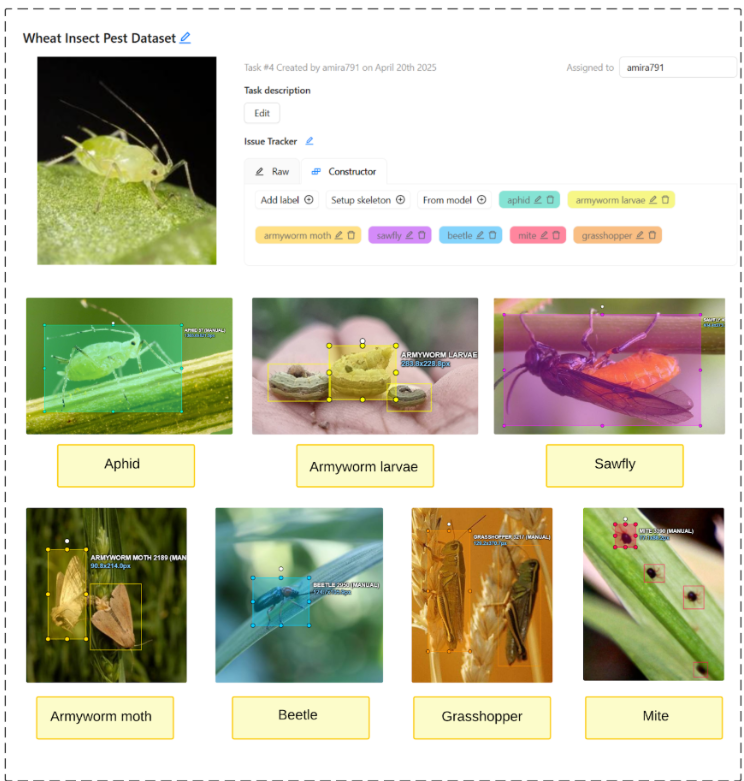
\includegraphics[width=0.9\textwidth]{chapters/chapter4/images/Figure08.png}
    \caption{Wheat insect pest annotation task in CVAT.}
    \label{fig:CVATAnnotation}
\end{figure}


\subsection{YOLOv8-OBB model used for insect pest detection}

To perform insect pest detection with greater precision, the YOLOv8-OBB model was selected due to its support for oriented bounding boxes (OBB). Unlike traditional regular bounding boxes, which align with the image axes and may not tightly fit irregular or rotated objects, OBBs allow for angled detection boxes that better conform to the actual shape and orientation of the target pests (see Figure 9 ). 

YOLOv8-OBB architecture is pre-trained and publicly available. This architecture is particularly well-suited for detecting pests that appear at various angles, orientations, and shapes in real-world field images. It follows the general structure of YOLOv8, consisting of:


\begin{itemize}
    \item \textbf{Backbone:} The backbone is responsible for extracting meaningful visual features from the input image. YOLOv8-OBB uses a CSPDarknet-inspired backbone, which combines convolutional layers, residual connections, and cross-stage partial connections (CSP).

    \item \textbf{Neck:} The Path Aggregation Network (PANet) is used to enhance and combine features from different depths of the backbone. It performs both bottom-up and top-down feature fusion, allowing:
    \begin{itemize}
        \item \textbf{Low-level features} (fine-grained texture, useful for small pests),
        \item \textbf{High-level features} (semantic information, useful for identifying object categories) to be merged effectively.
    \end{itemize}

    \item \textbf{Detection Head:} This is the main difference between YOLOv8 and YOLOv8-OBB.
    \begin{itemize}
        \item In standard YOLOv8, the detection head outputs a class label, objectness score, and four coordinates \((x, y, \text{width}, \text{height})\) for a regular bounding box.
        \item In YOLOv8-OBB, the detection head is modified to output eight coordinates representing a quadrilateral bounding box \((x_1, y_1, x_2, y_2, x_3, y_3, x_4, y_4)\). This allows the model to capture: \textit{rotation}, \textit{skewness}, and \textit{irregular shapes}. Such flexibility is particularly important in pest detection because:
        \begin{itemize}
            \item Pests can appear at arbitrary angles and orientations.
            \item The background (e.g., wheat leaves, stems) often causes overlap or partial occlusion.
            \item Regular bounding boxes tend to include excessive background or miss critical parts of the pest, reducing detection precision.
        \end{itemize}
        These limitations are visually illustrated in Figure~\ref{fig:obb_vs_hbb}, where it is evident that regular bounding boxes poorly fit rotated or elongated objects, while oriented bounding boxes provide tighter and more accurate localization. \parencite{ultralytics2024obb}. More details are presented in \ref{app:annexD}.
    \end{itemize}
\end{itemize}

\begin{figure}[H] % 'H' requires \usepackage{float}
    \centering
    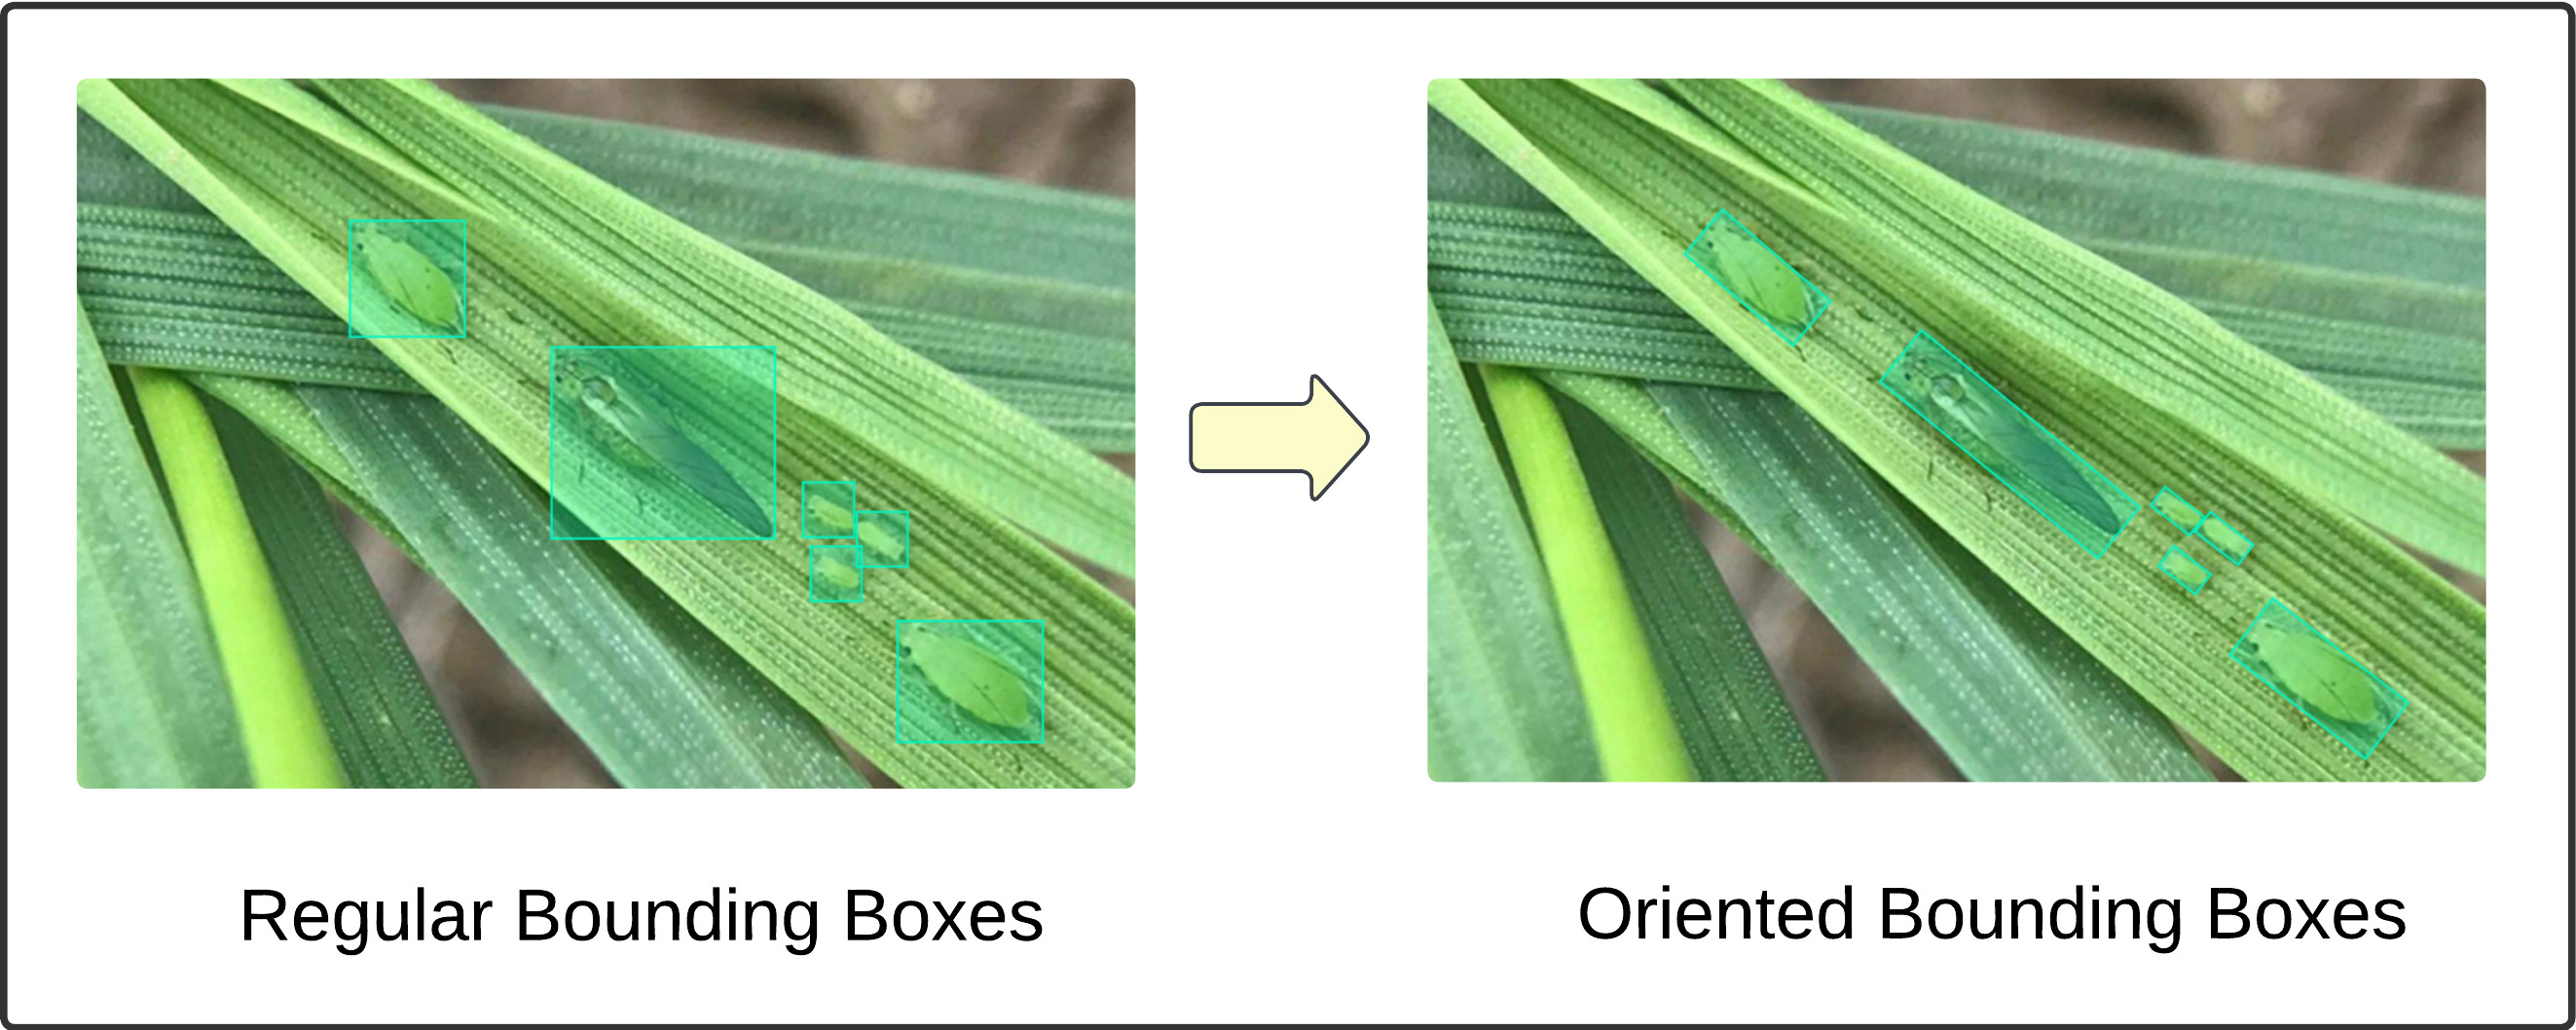
\includegraphics[width=0.9\textwidth]{chapters/chapter4/images/Figure13.jpeg}
    \caption{Comparison between regular bounding boxes and oriented bounding boxes.}
    \label{fig:obb_vs_hbb}
\end{figure}


    
\subsection{AI assistant integration for interactive agricultural intelligence}

To further enhance the usability and practical impact of the proposed system, an AI assistant module was integrated into the web application. This conversational interface allows farmers to interact naturally with the platform by submitting either text-based questions or images accompanied by a textual description. Users can inquire about wheat diseases, pest identifications, suitable treatments, or general agricultural best practices. By offering accurate and context-aware responses, the assistant bridges the gap between complex model outputs and user-friendly insights, enabling even non-expert users to make well-informed decisions quickly and confidently.

The chatbot was developed using the \textbf{Gemini API} on the \textbf{Google Cloud Platform (GCP)}. The Gemini large language model (LLM) offers advanced natural language processing capabilities, which are essential for understanding agricultural queries and generating detailed, helpful responses. In this system, the assistant handles two input types: 
\begin{itemize}
    \item Pure text queries—users may describe symptoms or ask for advice.
    \item Image uploads with a textual description—enabling more context-rich diagnosis, especially for disease or pest detection.
\end{itemize}

The back-end architecture ensures secure and efficient communication between the user interface and Gemini’s cloud-hosted model via API calls. Once a query is submitted, it is sent to Gemini’s inference endpoint, which returns a generated response in real time. This design allows the assistant to offer an interactive and intelligent experience embedded directly in the agricultural support platform. As visualized in the following figure~\ref{fig:ai_assistant_integration}, this integration empowers farmers to access actionable insights effortlessly—\textit{as presented in this figure}.

\begin{figure}[H] % 'H' requires \usepackage{float}
    \centering
    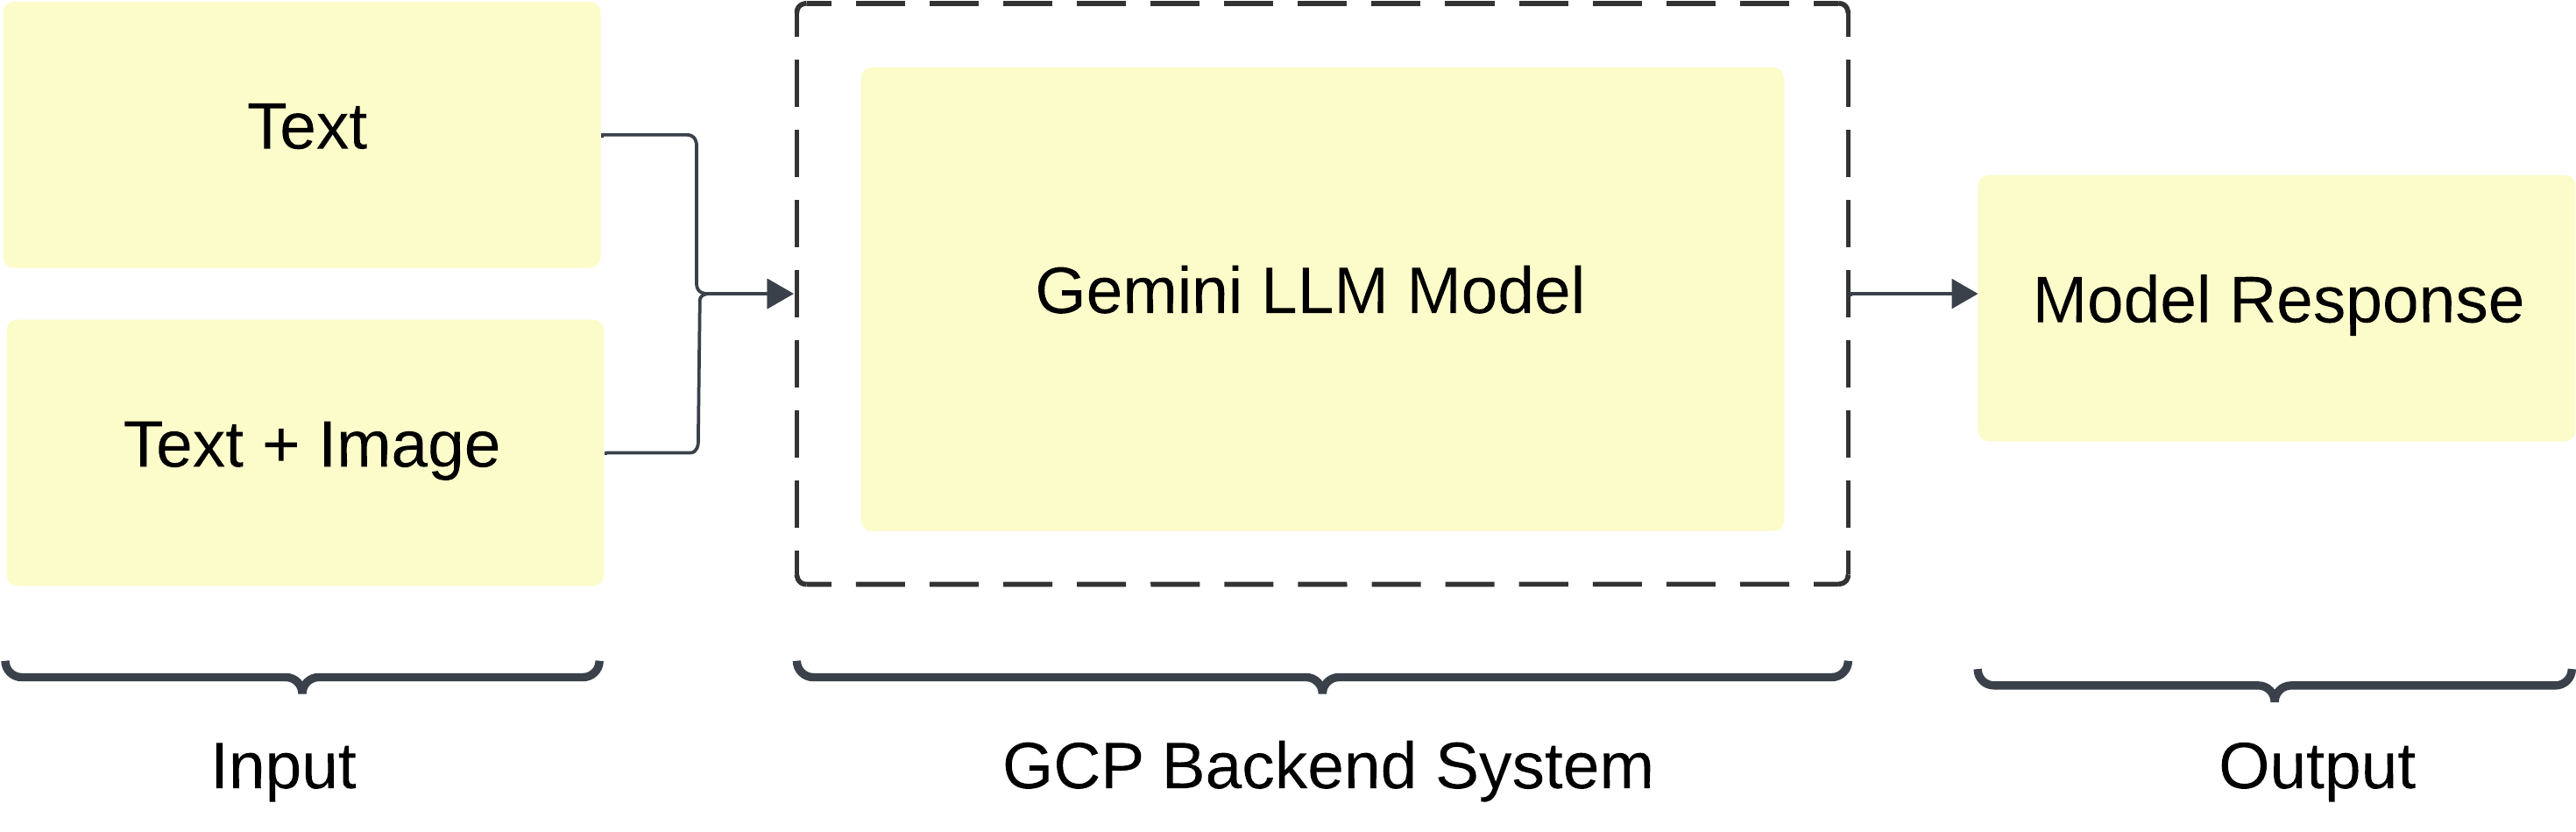
\includegraphics[width=0.9\textwidth]{chapters/chapter4/images/Figure14.png}
    \caption{AI assistant integration workflow.}
    \label{fig:ai_assistant_integration}
\end{figure}

\section{Web platform design}
To ensure practical usability of the proposed system by end users such as farmers, agronomists, and researchers, a dedicated web platform was developed. This platform serves as the main interface for interacting with the AI-based crop health monitoring system, integrating both wheat disease classification and insect pest detection modules.
The platform was designed with a focus on simplicity, efficiency, and accessibility, allowing users to upload images, receive predictions, and visualize results with minimal effort. 



\subsection{Functional Specifications}
The functional requirements of our system are detailed in the table below using the MoSCoW method (Must M, Should S, Could C, Won’t W) to prioritize features based on their importance. This system is designed to assist farmers in classifying wheat diseases and identifying insect pests through an easy-to-use web application (see Table~\ref{tab:FunctionalSpecifications}).


\begin{table}[h!]
\centering
\caption{Functional specifications of the web platform}
\begin{tabular}{|c|p{12cm}|c|}
\hline
\textbf{ID} & \textbf{Requirement} & \textbf{Priority} \\
\hline
F1 & The system must allow the user to upload images and analyze them. & M \\
\hline
F2 & The system must allow the user to select a prediction task (Wheat disease classification, Insect pest detection). & M \\
\hline
F3 & The system must allow the user to visualize the result of the prediction, including annotated images and relevant classification or detection details. & M \\
\hline
F4 & The system must process the image using the appropriate trained model and display the prediction results. & M \\
\hline
F5 & The system must allow users to export(download) prediction result. & M \\
\hline
F6 & The system should provide a chatbot assistant to guide and support the user. & S \\
\hline
F7 & The system could provide a documentation section containing detailed descriptions of common wheat diseases and insect pests, including symptoms, impact, and treatment suggestions. & C \\
\hline
\end{tabular}
\label{tab:FunctionalSpecifications}
\end{table}



\subsection{Use case diagrams}
The use case diagram is a diagram used to model the needs of users and provide an overall view of the system's functionalities. It is based on UML use case diagrams. Figure~\ref{fig:usecase} presents the use case diagram of our software prototype.The primary user of the system is the farmer, responsible for interacting with its functionalities to monitor wheat health, identify pests, and receive predictions. 




\begin{figure}[H] % 'H' needs \usepackage{float}
    \centering
    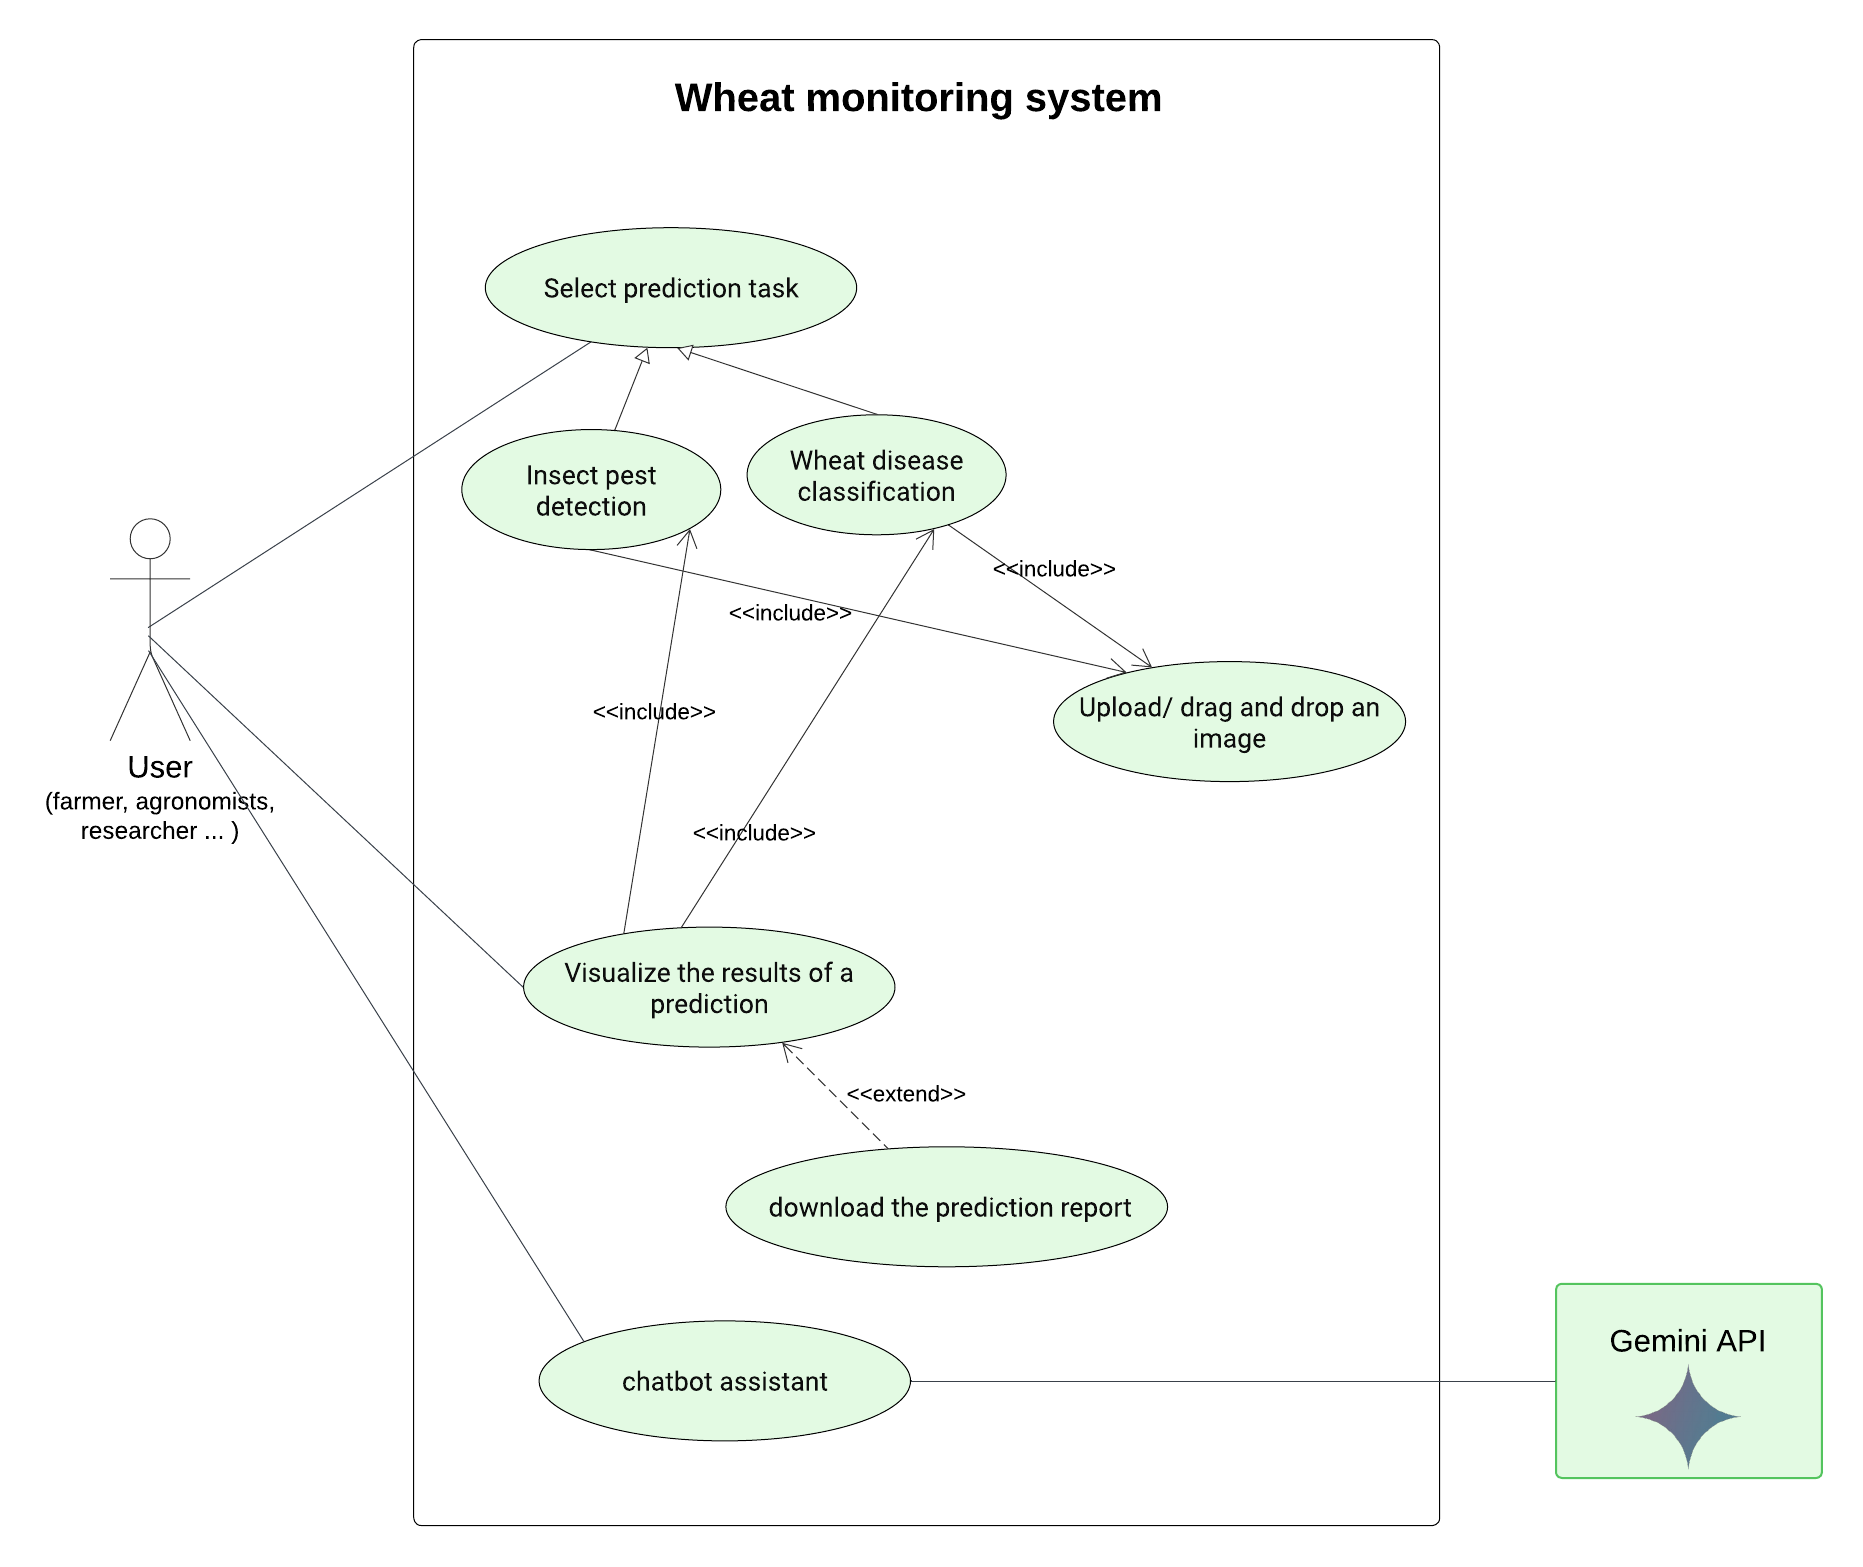
\includegraphics[width=0.9\textwidth]{chapters/chapter4/images/Figure10.png}
    \caption{The use case diagram of the system.}
    \label{fig:usecase}
\end{figure}

\subsection{Activity diagrams}

Activity diagrams provide a high-level view of the dynamic behavior of the system. They are particularly useful for illustrating the sequence of actions involved in performing specific tasks from a user perspective. In the context of our web platform, we developed two distinct activity diagrams (Figure~\ref{fig:ActivityDiagrams}), each corresponding to a core task of the system: wheat disease classification and wheat insect pest detection. These diagrams help visualize the user interaction flow, system responses, and processing steps for each use case. (see Figure~\ref{fig:usecase})


\begin{figure}[H] % 'H' needs \usepackage{float}
    \centering
    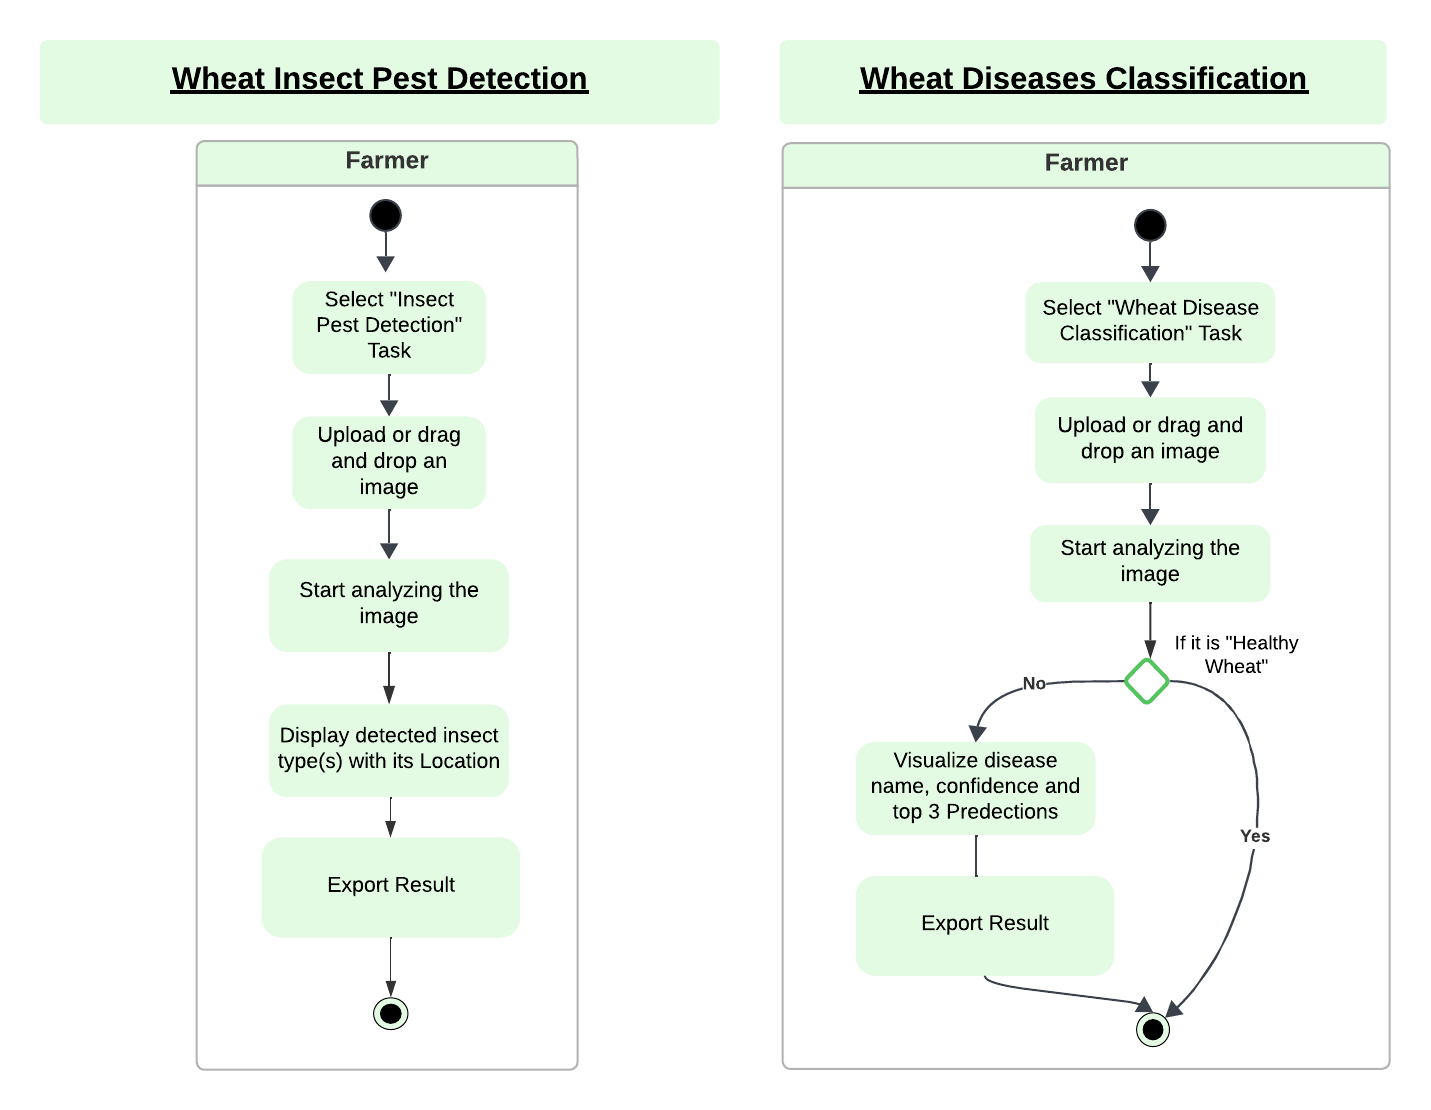
\includegraphics[width=\textwidth]{chapters/chapter4/images/Figure12.png}
    \caption{Activity diagrams for Wheat disease classification and insect pest detection}
    \label{fig:ActivityDiagrams}
\end{figure}


% \begin{figure}[H] % 'H' needs \usepackage{float}
%     \centering
%     
\includegraphics[width=0.9\textwidth]{chapters/chapter4/images/Figure11.png}
%     \caption{Activity Diagram for Wheat Disease Classification.}
%     \label{fig:ActivityDiagramWheat}
% \end{figure}



% \begin{figure}[H] % 'H' needs \usepackage{float}
%     \centering
%     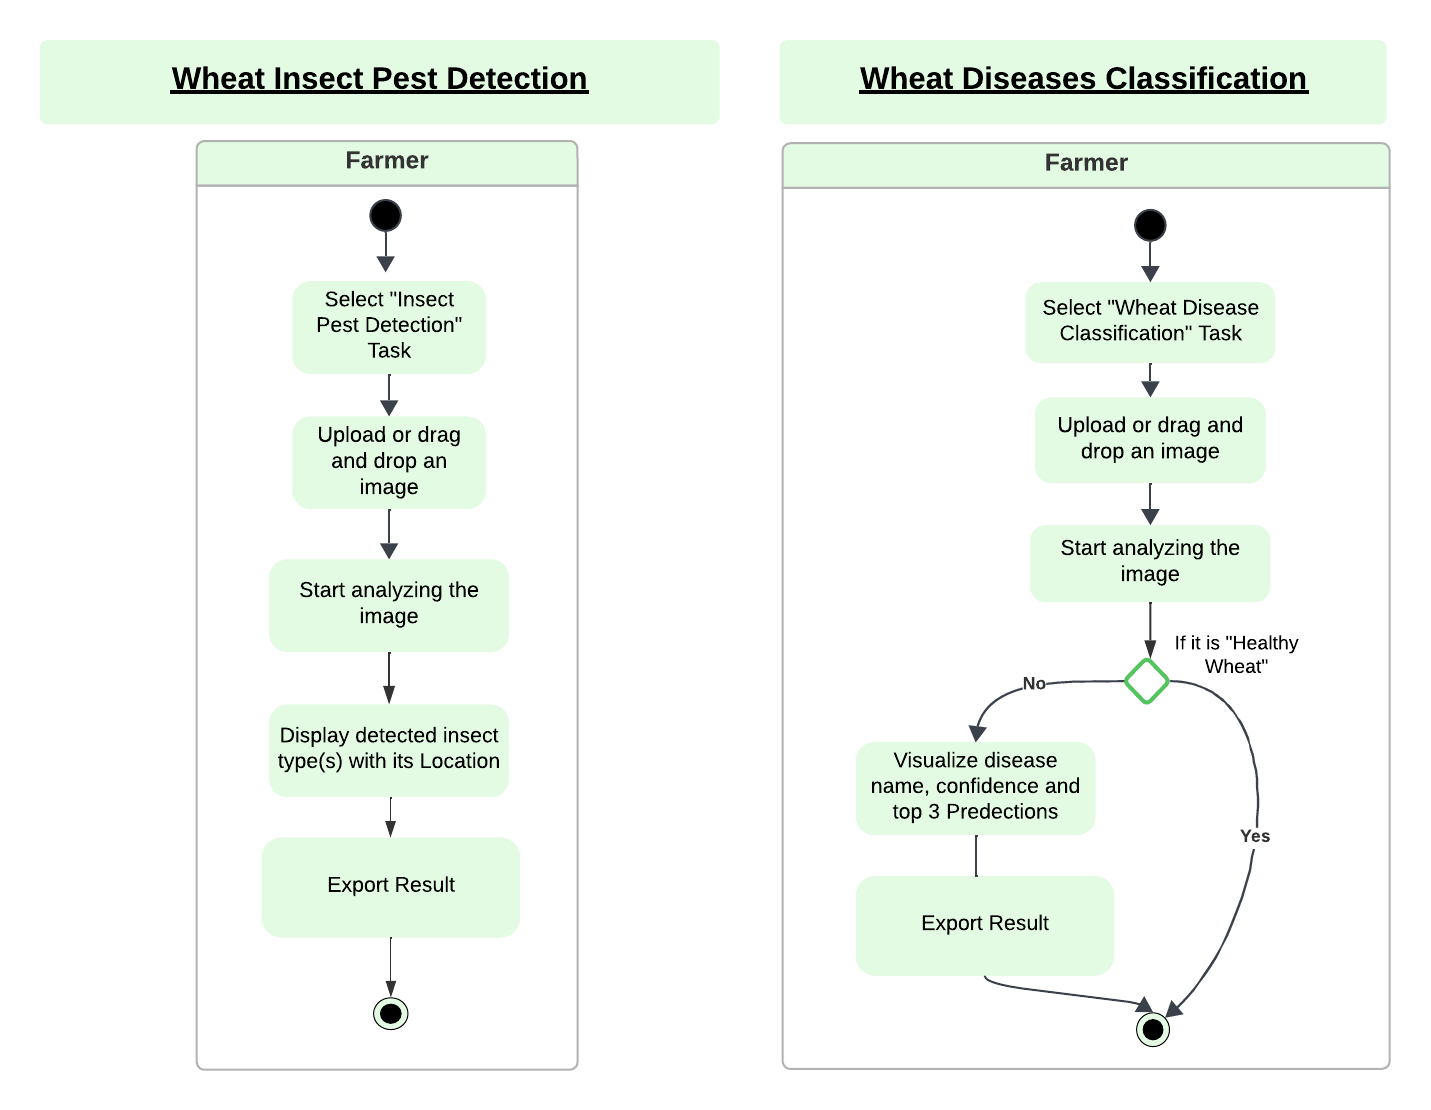
\includegraphics[width=0.9\textwidth]{chapters/chapter4/images/Figure12.png}
%     \caption{Activity Diagram for Wheat Insect Pest Detection.}
%     \label{fig:ActivityDiagramPest}
% \end{figure}


\section{Conclusion}
This chapter details the design of our proposed system for wheat disease classification and pest detection, emphasizing the integration of advanced deep learning models and carefully constructed datasets. The architecture and web platform design lay a solid foundation for practical deployment, ensuring usability and accuracy. The next chapter will focus on the implementation aspects, translating this design into a functional prototype and evaluating its performance in real-world scenarios.